\documentclass[border=8pt]{standalone}
\usepackage[T1]{fontenc}
\usepackage{amsmath,amssymb}
\usepackage{tikz}
\usetikzlibrary{arrows.meta,calc}
\renewcommand{\familydefault}{\sfdefault}

\definecolor{kthblue}{HTML}{004791}
\definecolor{kthlight}{HTML}{DEF0FC}
\definecolor{kthorange}{HTML}{E37222}
\definecolor{kthdark}{HTML}{000061}
\definecolor{kthmid}{HTML}{6298D2}
\definecolor{kthgreen}{HTML}{3F8F4F}

\newcommand{\bV}{\mathbf{V}}
\newcommand{\bU}{\mathbf{U}}
\newcommand{\bH}{\mathbf{H}}
\newcommand{\bn}{\mathbf{n}}

\begin{document}
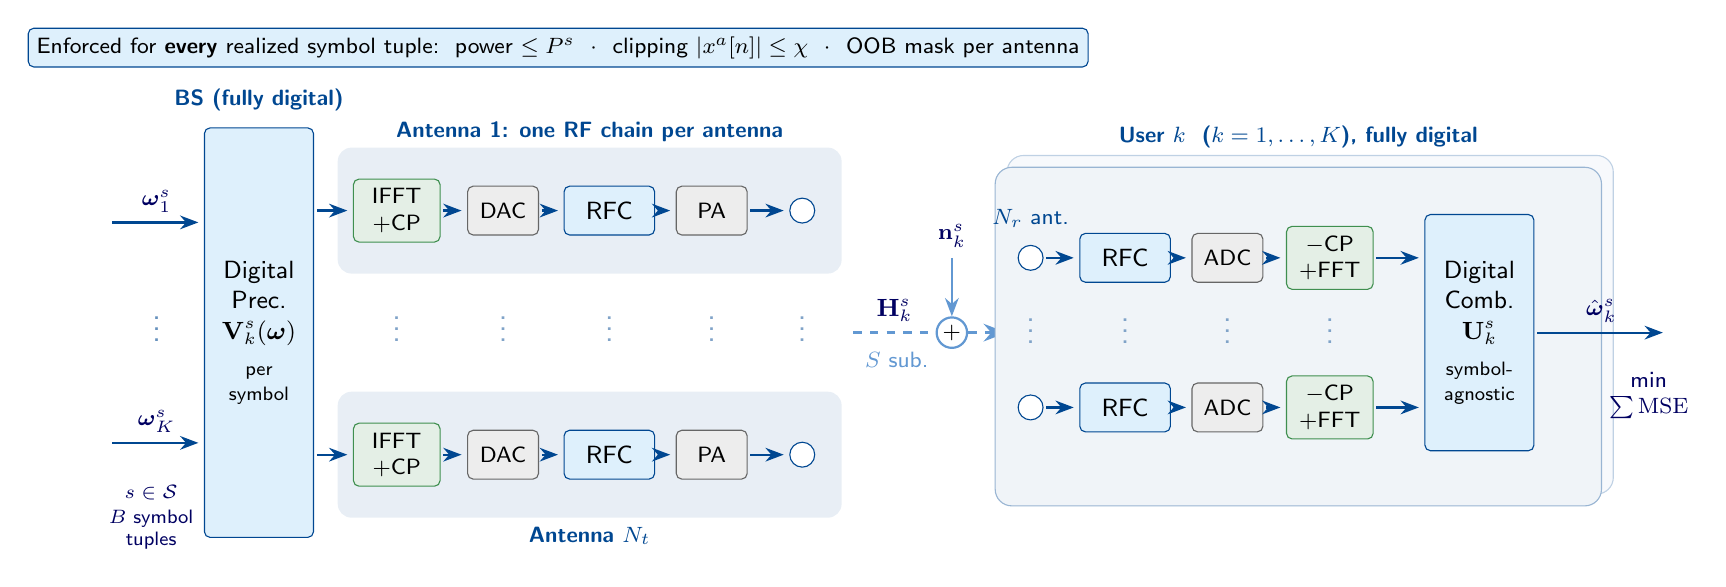
\begin{tikzpicture}[
    font=\small, x=1cm, y=1cm,
    rfc/.style={draw=kthblue,fill=kthlight,rounded corners=2pt,minimum width=1.15cm,minimum height=0.62cm,align=center,font=\small},
    ofdm/.style={draw=kthgreen,fill=kthgreen!14,rounded corners=2pt,minimum width=1.10cm,minimum height=0.80cm,align=center,font=\footnotesize,inner sep=1pt},
    conv/.style={draw=black!60,fill=black!7,rounded corners=2pt,minimum width=0.90cm,minimum height=0.62cm,align=center,font=\footnotesize},
    ant/.style={draw=kthblue,fill=white,circle,inner sep=0pt,minimum size=9pt},
    arr/.style={->,>=Stealth,thick,kthblue,shorten <=1pt,shorten >=2pt},
    cnote/.style={font=\footnotesize,draw=kthblue,fill=kthlight,rounded corners=2pt,inner sep=3pt,align=center},
    ]

    % ---------------- BS (fully digital) ----------------
    \node[rfc, minimum height=5.2cm, minimum width=1.35cm, text width=1.15cm] (dig) at (0.75,0)
        {Digital\\Prec.\\$\bV_k^s(\boldsymbol{\omega})$\\[2pt]{\scriptsize per}\\[-2pt]{\scriptsize symbol}};
    \node[font=\footnotesize\bfseries,kthblue,above=0.08cm] at (dig.north){BS (fully digital)};
    \draw[arr](-1.15,1.40)--node[above,font=\footnotesize,kthdark]{$\boldsymbol{\omega}_1^s$}(dig.west|-0,1.40);
    \draw[arr](-1.15,-1.40)--node[above,font=\footnotesize,kthdark]{$\boldsymbol{\omega}_K^s$}(dig.west|-0,-1.40);
    \node[kthblue!60,font=\large] at (-0.55,0.15){$\vdots$};
    \node[font=\scriptsize,kthdark,align=center] at (-0.62,-2.35){$s\in\mathcal{S}$\\[1pt]$B$ symbol\\tuples};

    \node[cnote] at (4.55,3.62)
        {Enforced for \textbf{every} realized symbol tuple:\ \ power $\le P^s$ \ $\cdot$ \ clipping $|x^a[n]|\le\chi$ \ $\cdot$ \ OOB mask per antenna};

    \fill[kthblue!9,rounded corners=5pt] (1.75,0.75) rectangle (8.15,2.35);
    \fill[kthblue!9,rounded corners=5pt] (1.75,-2.35) rectangle (8.15,-0.75);
    \node[font=\footnotesize\bfseries,kthblue] at (4.95,2.55){Antenna 1: one RF chain per antenna};
    \node[font=\footnotesize\bfseries,kthblue] at (4.95,-2.58){Antenna $N_t$};

    \foreach \y/\lab in {1.55/a, -1.55/b}{
        \node[ofdm] (ifft\lab) at (2.50,\y){IFFT\\+CP};
        \node[conv] (dac\lab)  at (3.85,\y){DAC};
        \node[rfc]  (rfc\lab)  at (5.20,\y){RFC};
        \node[conv] (pa\lab)   at (6.50,\y){PA};
        \node[ant]  (ant\lab)  at (7.65,\y){};
        \draw[arr](dig.east|-ifft\lab)--(ifft\lab.west);
        \draw[arr](ifft\lab.east)--(dac\lab.west);
        \draw[arr](dac\lab.east)--(rfc\lab.west);
        \draw[arr](rfc\lab.east)--(pa\lab.west);
        \draw[arr](pa\lab.east)--(ant\lab.west);
    }
    \foreach \x in {2.50,3.85,5.20,6.50,7.65}{\node[kthblue!50,font=\large] at (\x,0.15){$\vdots$};}

    % ---------------- channel + noise ----------------
    \node[draw=kthmid,thick,circle,inner sep=0pt,minimum size=11pt,font=\footnotesize] (sum) at (9.55,0){$+$};
    \draw[kthmid,dashed,very thick](8.30,0)--node[above,font=\small,kthdark]{$\bH_k^s$}(sum.west);
    \node[font=\footnotesize,kthmid,below=0.12cm] at (8.85,0){$S$ sub.};
    \draw[->,>=Stealth,thick,kthmid](9.55,0.95)node[above,font=\footnotesize,kthdark]{$\bn_k^s$}--(sum.north);
    \draw[->,>=Stealth,kthmid,dashed,very thick](sum.east)--(10.25,0);

    % ---------------- user k (fully digital) ----------------
    \fill[kthblue!3,rounded corners=6pt,draw=kthblue!25] (10.25,-2.05) rectangle (17.95,2.25);
    \fill[kthblue!6,rounded corners=6pt,draw=kthblue!40] (10.10,-2.20) rectangle (17.80,2.10);
    \node[font=\footnotesize\bfseries,kthblue] at (13.95,2.48){User $k$ \ ($k=1,\dots,K$), fully digital};

    \foreach \y/\lab in {0.95/a, -0.95/b}{
        \node[ant]  (rx\lab)   at (10.55,\y){};
        \node[rfc]  (urfc\lab) at (11.75,\y){RFC};
        \node[conv] (adc\lab)  at (13.05,\y){ADC};
        \node[ofdm] (fft\lab)  at (14.35,\y){$-$CP\\+FFT};
        \draw[arr](rx\lab.east)--(urfc\lab.west);
        \draw[arr](urfc\lab.east)--(adc\lab.west);
        \draw[arr](adc\lab.east)--(fft\lab.west);
    }
    \foreach \x in {10.55,11.75,13.05,14.35}{\node[kthblue!50,font=\large] at (\x,0.12){$\vdots$};}
    \node[font=\footnotesize,kthblue] at (10.55,1.45){$N_r$ ant.};

    \node[rfc,minimum height=3.0cm,minimum width=1.35cm,text width=1.15cm] (udig) at (16.25,0)
        {Digital\\Comb.\\$\bU_k^s$\\[2pt]{\scriptsize symbol-}\\[-2pt]{\scriptsize agnostic}};
    \draw[arr](ffta.east)--(udig.west|-ffta);
    \draw[arr](fftb.east)--(udig.west|-fftb);
    \draw[arr](udig.east)--node[above,font=\footnotesize,kthdark]{$\hat{\boldsymbol{\omega}}_k^s$}(18.65,0);
    \node[font=\footnotesize,kthdark,align=center] at (18.40,-0.80){min\\$\sum\mathrm{MSE}$};
\end{tikzpicture}
\end{document}
